\chapter{検証}
\label{chap:poordirection}


\section{検証1}

\subsection{検証背景}

\subsubsection{検証目的}

password認証方式の,新規登録・認証の面倒さを解決するために,第3章の提案手法で
password認証方式に変わる,公開鍵暗号方式によるssh認証を用いた,WEBサービス認証の提案を行った。\\
しかしながら,提案だけだと,新規登録・認証の面倒さを解決していることの根拠に乏しい。
よって,検証を行い,第3章の提案手法は"面倒さの軽減"に効果的に繋がっているかの確認をする。


\subsubsection{検証手段}

検証の手段としては,実際に,以下の2っの認証方式の登録・認証を被験者に体験してもらう。
%また,実験マニュアルを作成し,実験者は被験者に対して,同じように接するようにする。

\begin{itemize}
  \item パスワード方式認証(以後 "パスワード認証"と記述する)
  \item 公開鍵暗号暗号方式によるssh認証(以後 "鍵認証”と記述する)
\end{itemize}
その後,2っの観点から,"面倒さ"を数値化する。

1っ目の観点は「時間」である。
"面倒さ"をアカウント登録・認証にかかる時間と推測し,計測化する。
詳しい詳細については,検証環境のマニュアルに記述する。

%まず,パスワード 形式による登録・認証の時間計測をそれぞれ行う。
% 次に,公開鍵暗号方式によるSSH 形式登録・認証の時間計測をそれぞれ行う。
% 最後に,上記の形式による時間計測を比較する。

2っ目の観点は「アンケート」である。
アンケートには,点数で答える方式,文字で記入する欄 の2っがあり,点数で答える方式により"面倒さ”を数値化する。
アンケートの細かい内容は,4.1.3の検証画面に記述する。

また,アンケートには"面倒さ"を数値化する以外にも,以下の2っの意味を込める。
1っ目の意味は次の通りである。
アカウント登録・認証にかかる時間 を,"面倒さ"と予想して検証しているが,その予想を確かめる必要がある。
アンケートを取ることにより,「アカウント登録・認証にかかる時間」と,「アンケートによる面倒さ」が比例していることを確認することで,予想を確かめることができる。
また,被験者の状態も確認することで,面倒と感じるのが,検証自体に対しての面倒さと関係があるのかを確認する。
2っ目の意味は次のとおりである。
記入欄で,改善点や感じたことの意見をもらうことで,今後の研究に生きるようなアンケートをもらう。








\subsection{検証環境}
 \subsubsection{検証場所}
 第3章で記述したとおり,検証場所は学科のVMを用いているため,学科のネットワーク内(有線LAN,wifiアクセスポイント{ie-ryukyu})
 から,アクセスして検証を行う。


 %\subsubsection{検証画面}

 \subsubsection{検証の流れ}
    ここでは,被験者に行ってもらう,検証の流れを記述する。
    時間の観点で"面倒さ"を数値化する検証では,被験者にはパスワード方式,鍵方式の登録・認証をそれぞれ行ってもらう。その時,被験者は時間を測る。 
    また,再現性を持って,検証を行うためにマニュアルを作成し,マニュアル通りに検証を行う。
    アンケートの観点で"面倒さ"を数値化する検証では,
    時間の観点で"面倒さ"を数値化する検証 が終わった直後に行うようにすることで,被験者の思った感情とアンケート結果の差異が少なくなるようにする。
  

  \subsubsection{検証画面}
    %実際に記述--------------------------------------------------------
    ここでは,被験者に行ったもらう検証画面をのせる。

    以下の
    図\ref{検証1アカウント作成(パスワード方式)},
    図\ref{検証1認証(パスワード方式)}
    図\ref{検証1認証成功後(パスワード方式)}
    は,第3章の提案手法で実現したパスワード方式,登録・認証を,実際に被験者に行ってもらった時のブラウザ画面である。
    図\ref{検証1アカウント作成(パスワード方式)}は,アカウント登録画面である。
    図\ref{検証1認証(パスワード方式)}は,図\ref{検証1アカウント作成(パスワード方式)}で登録したアカウントに認証するための画面である。
    図\ref{検証1認証成功後(パスワード方式)}は,図\ref{検証1認証(パスワード方式)}で認証成功した後の画面である。
    % パスワード方式のスクショ---------------------------
    \vspace{4cm}%図の位置を正しくする!
    %\begin{figure}[h]
    \begin{figure}[H]
        %\centering
        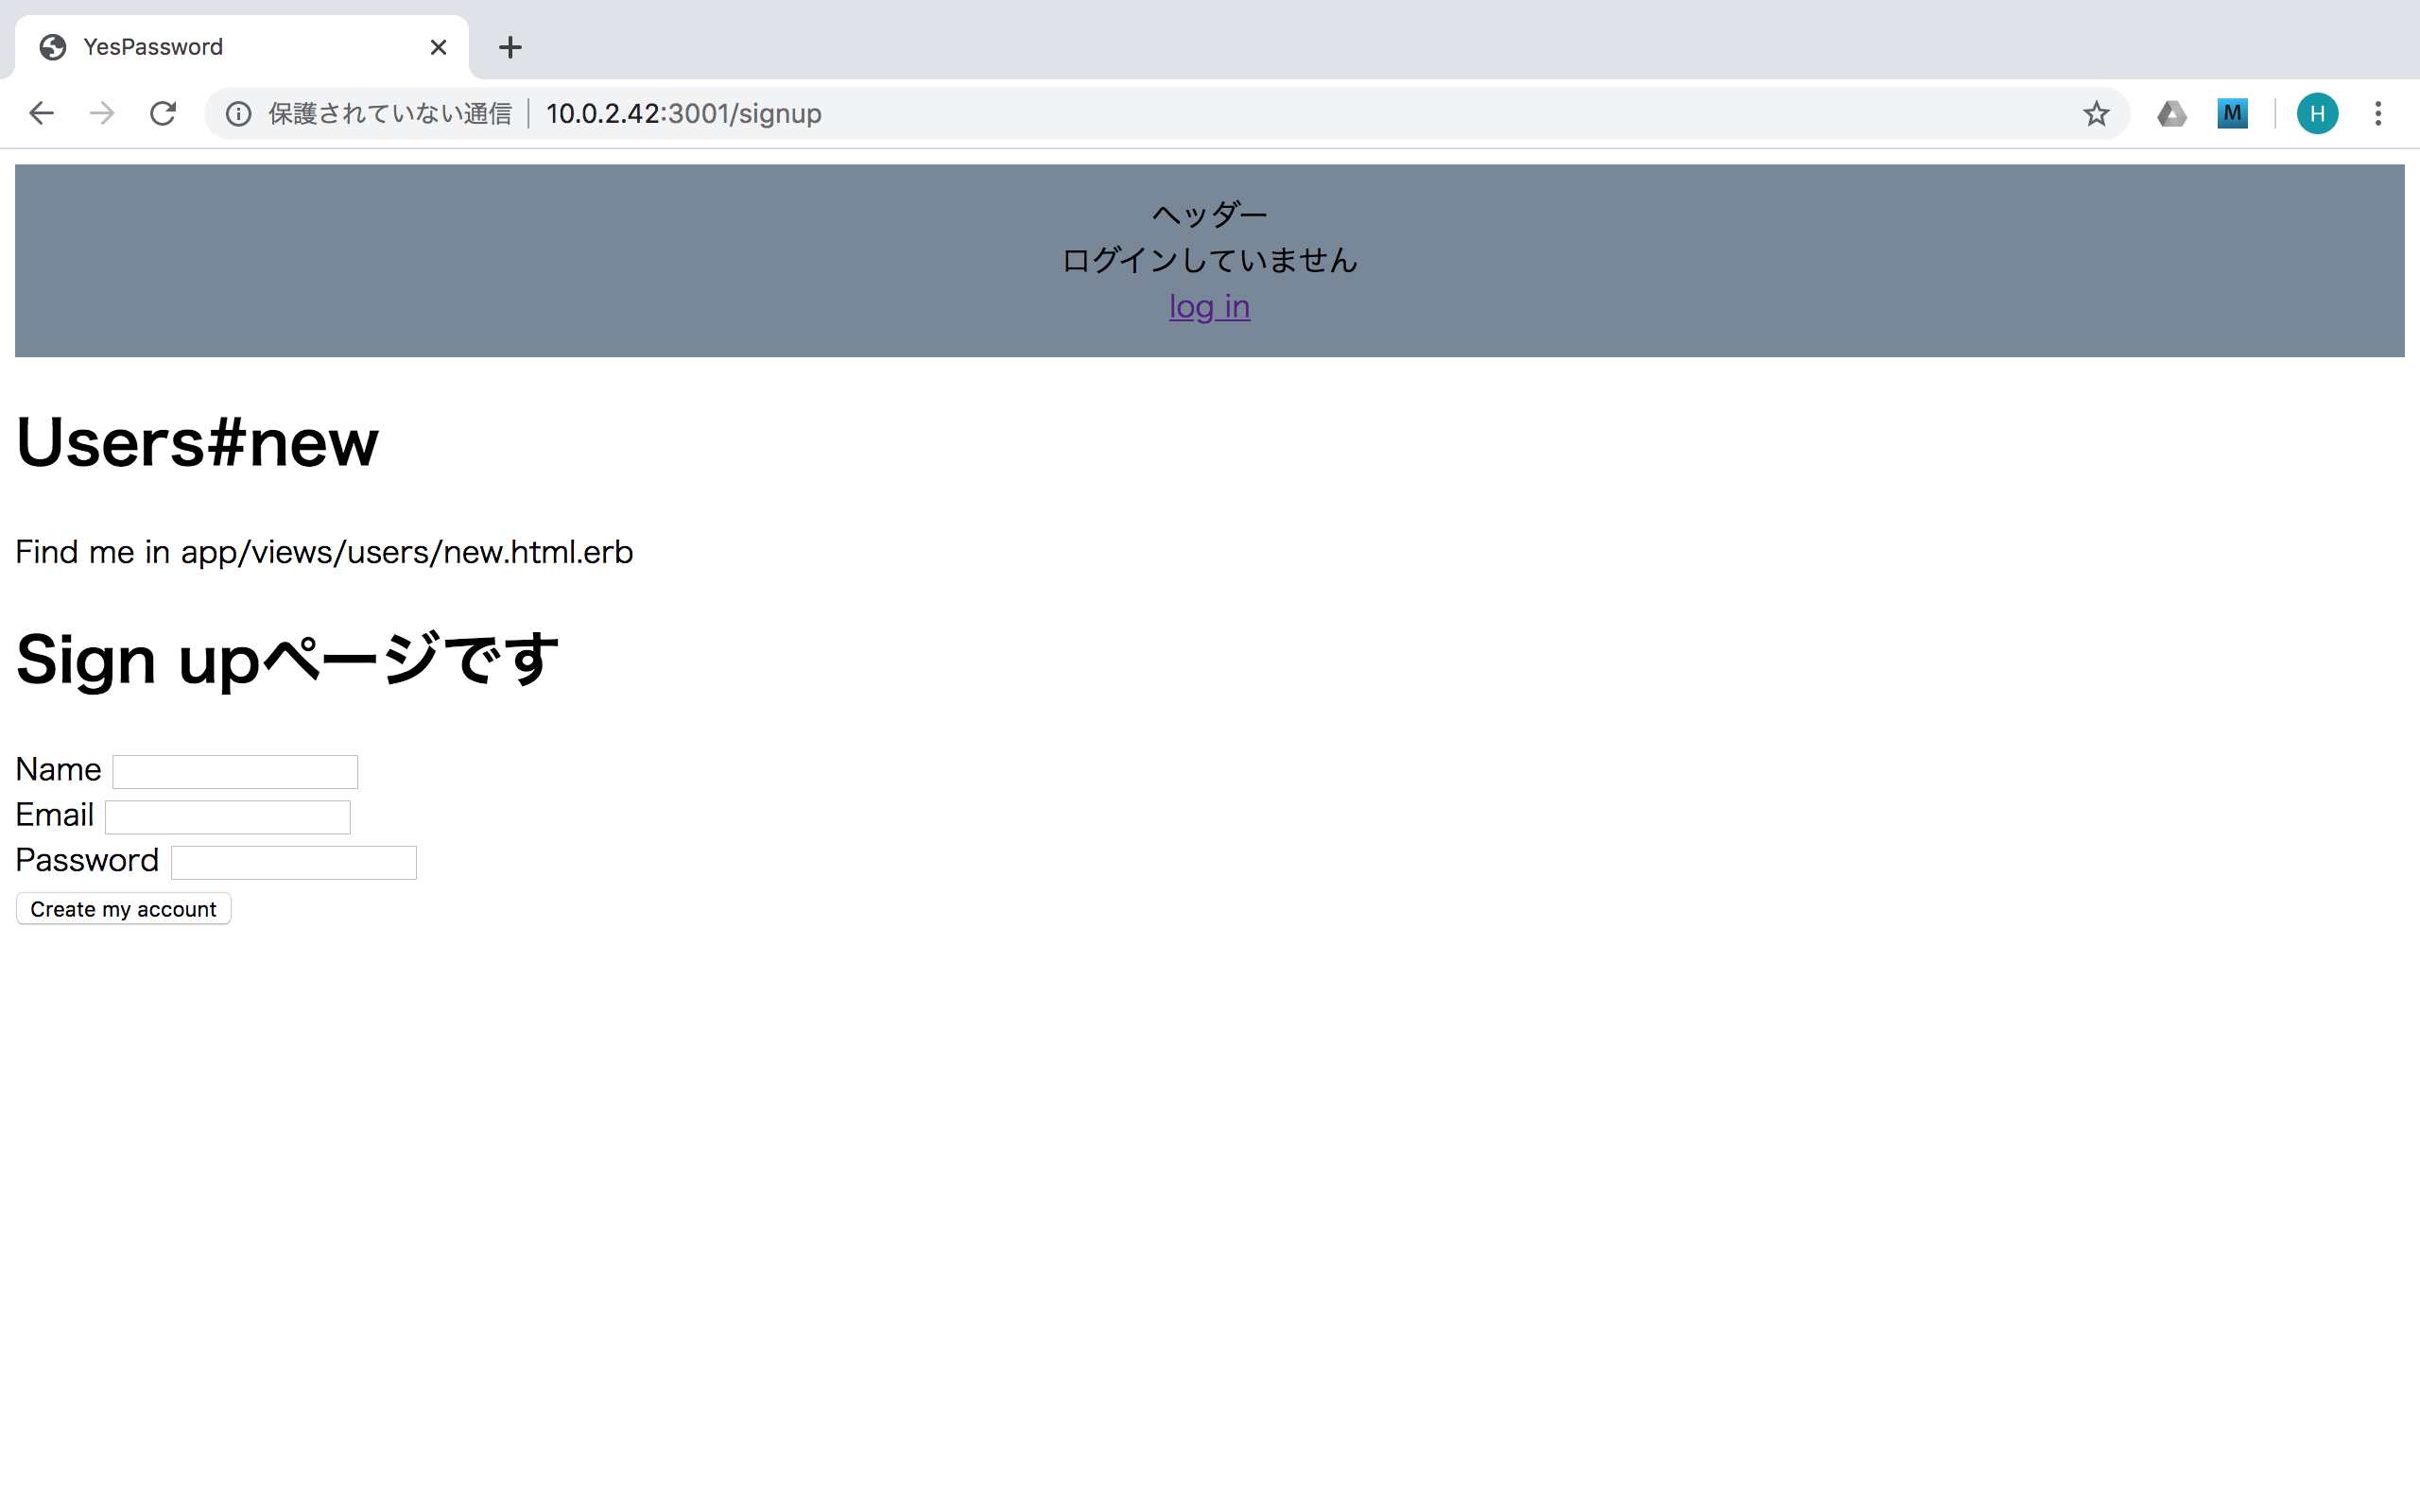
\includegraphics[width=15cm]{./fig/chapter4/inspect_1/password_screnn/sign_up.png}
        \caption{検証1\_アカウント作成(パスワード方式)}
        \label{検証1アカウント作成(パスワード方式)}
    \end{figure}

    \vspace{4cm}%図の位置を正しくする!
    \begin{figure}[H]
        %\centering
        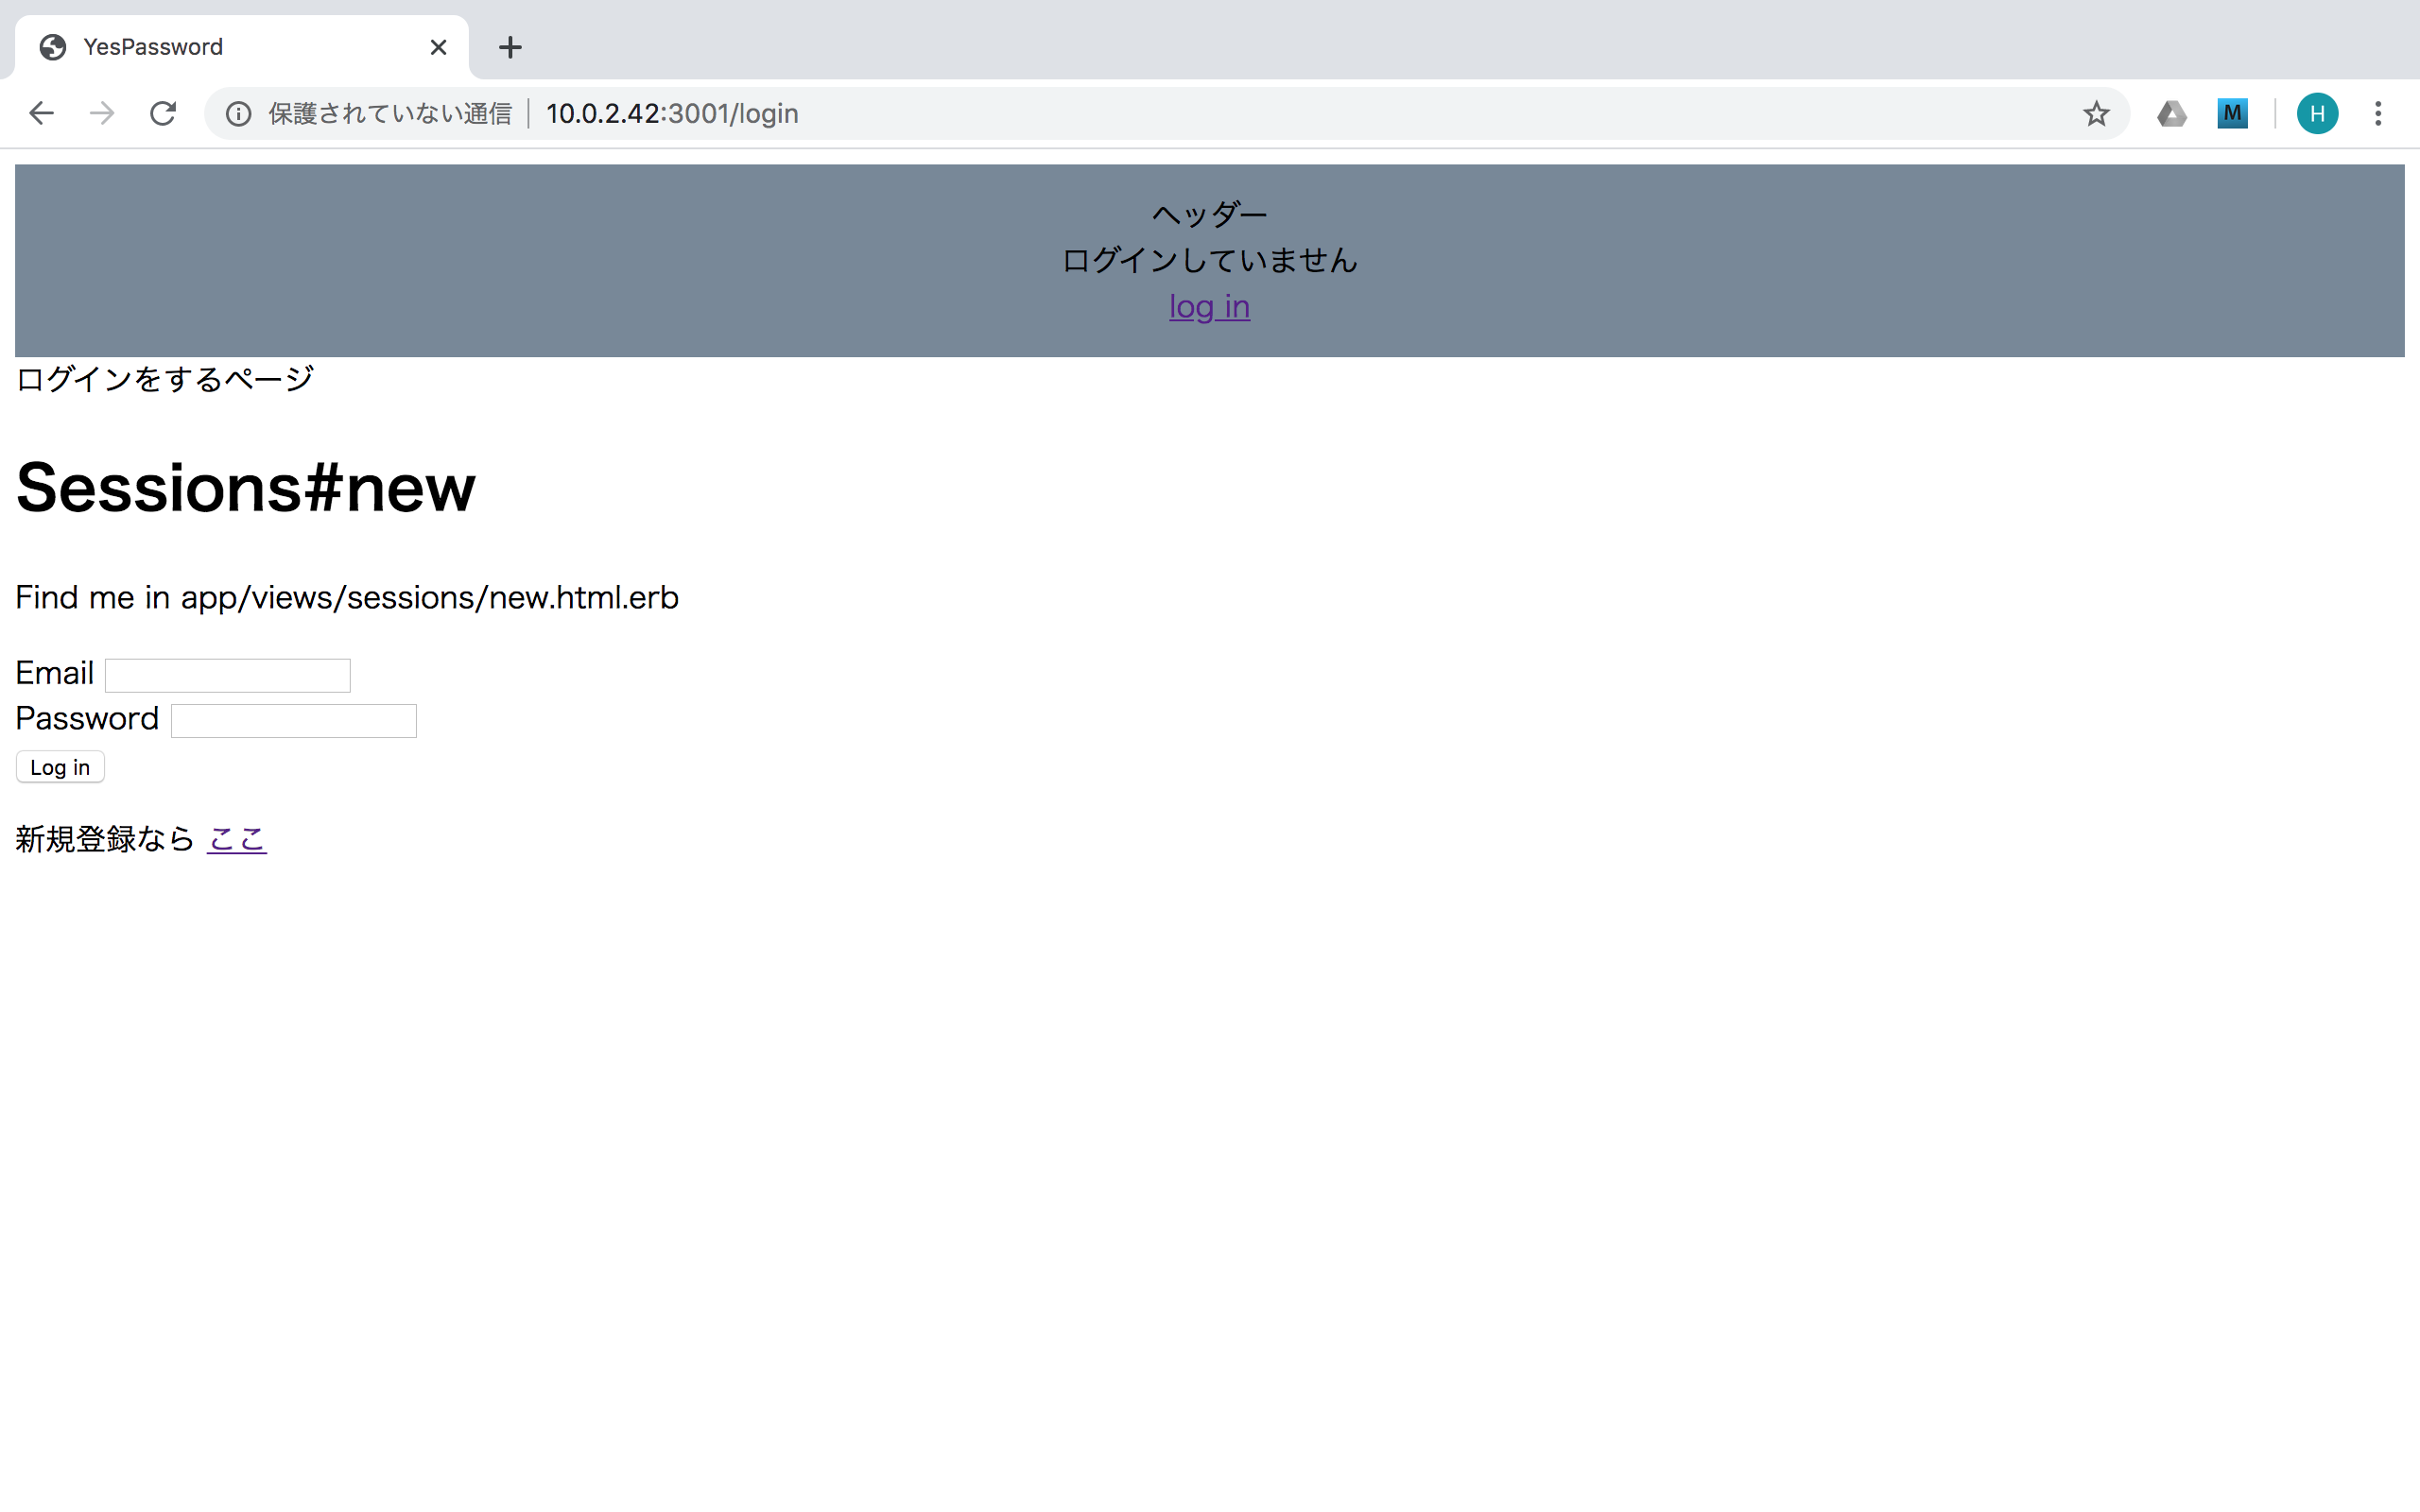
\includegraphics[width=15cm]{./fig/chapter4/inspect_1/password_screnn/login.png}
        \caption{検証1\_認証(パスワード方式)}
        \label{検証1認証(パスワード方式)}
    \end{figure}

    \vspace{4cm}%図の位置を正しくする!
    \begin{figure}[H]
        %\centering
        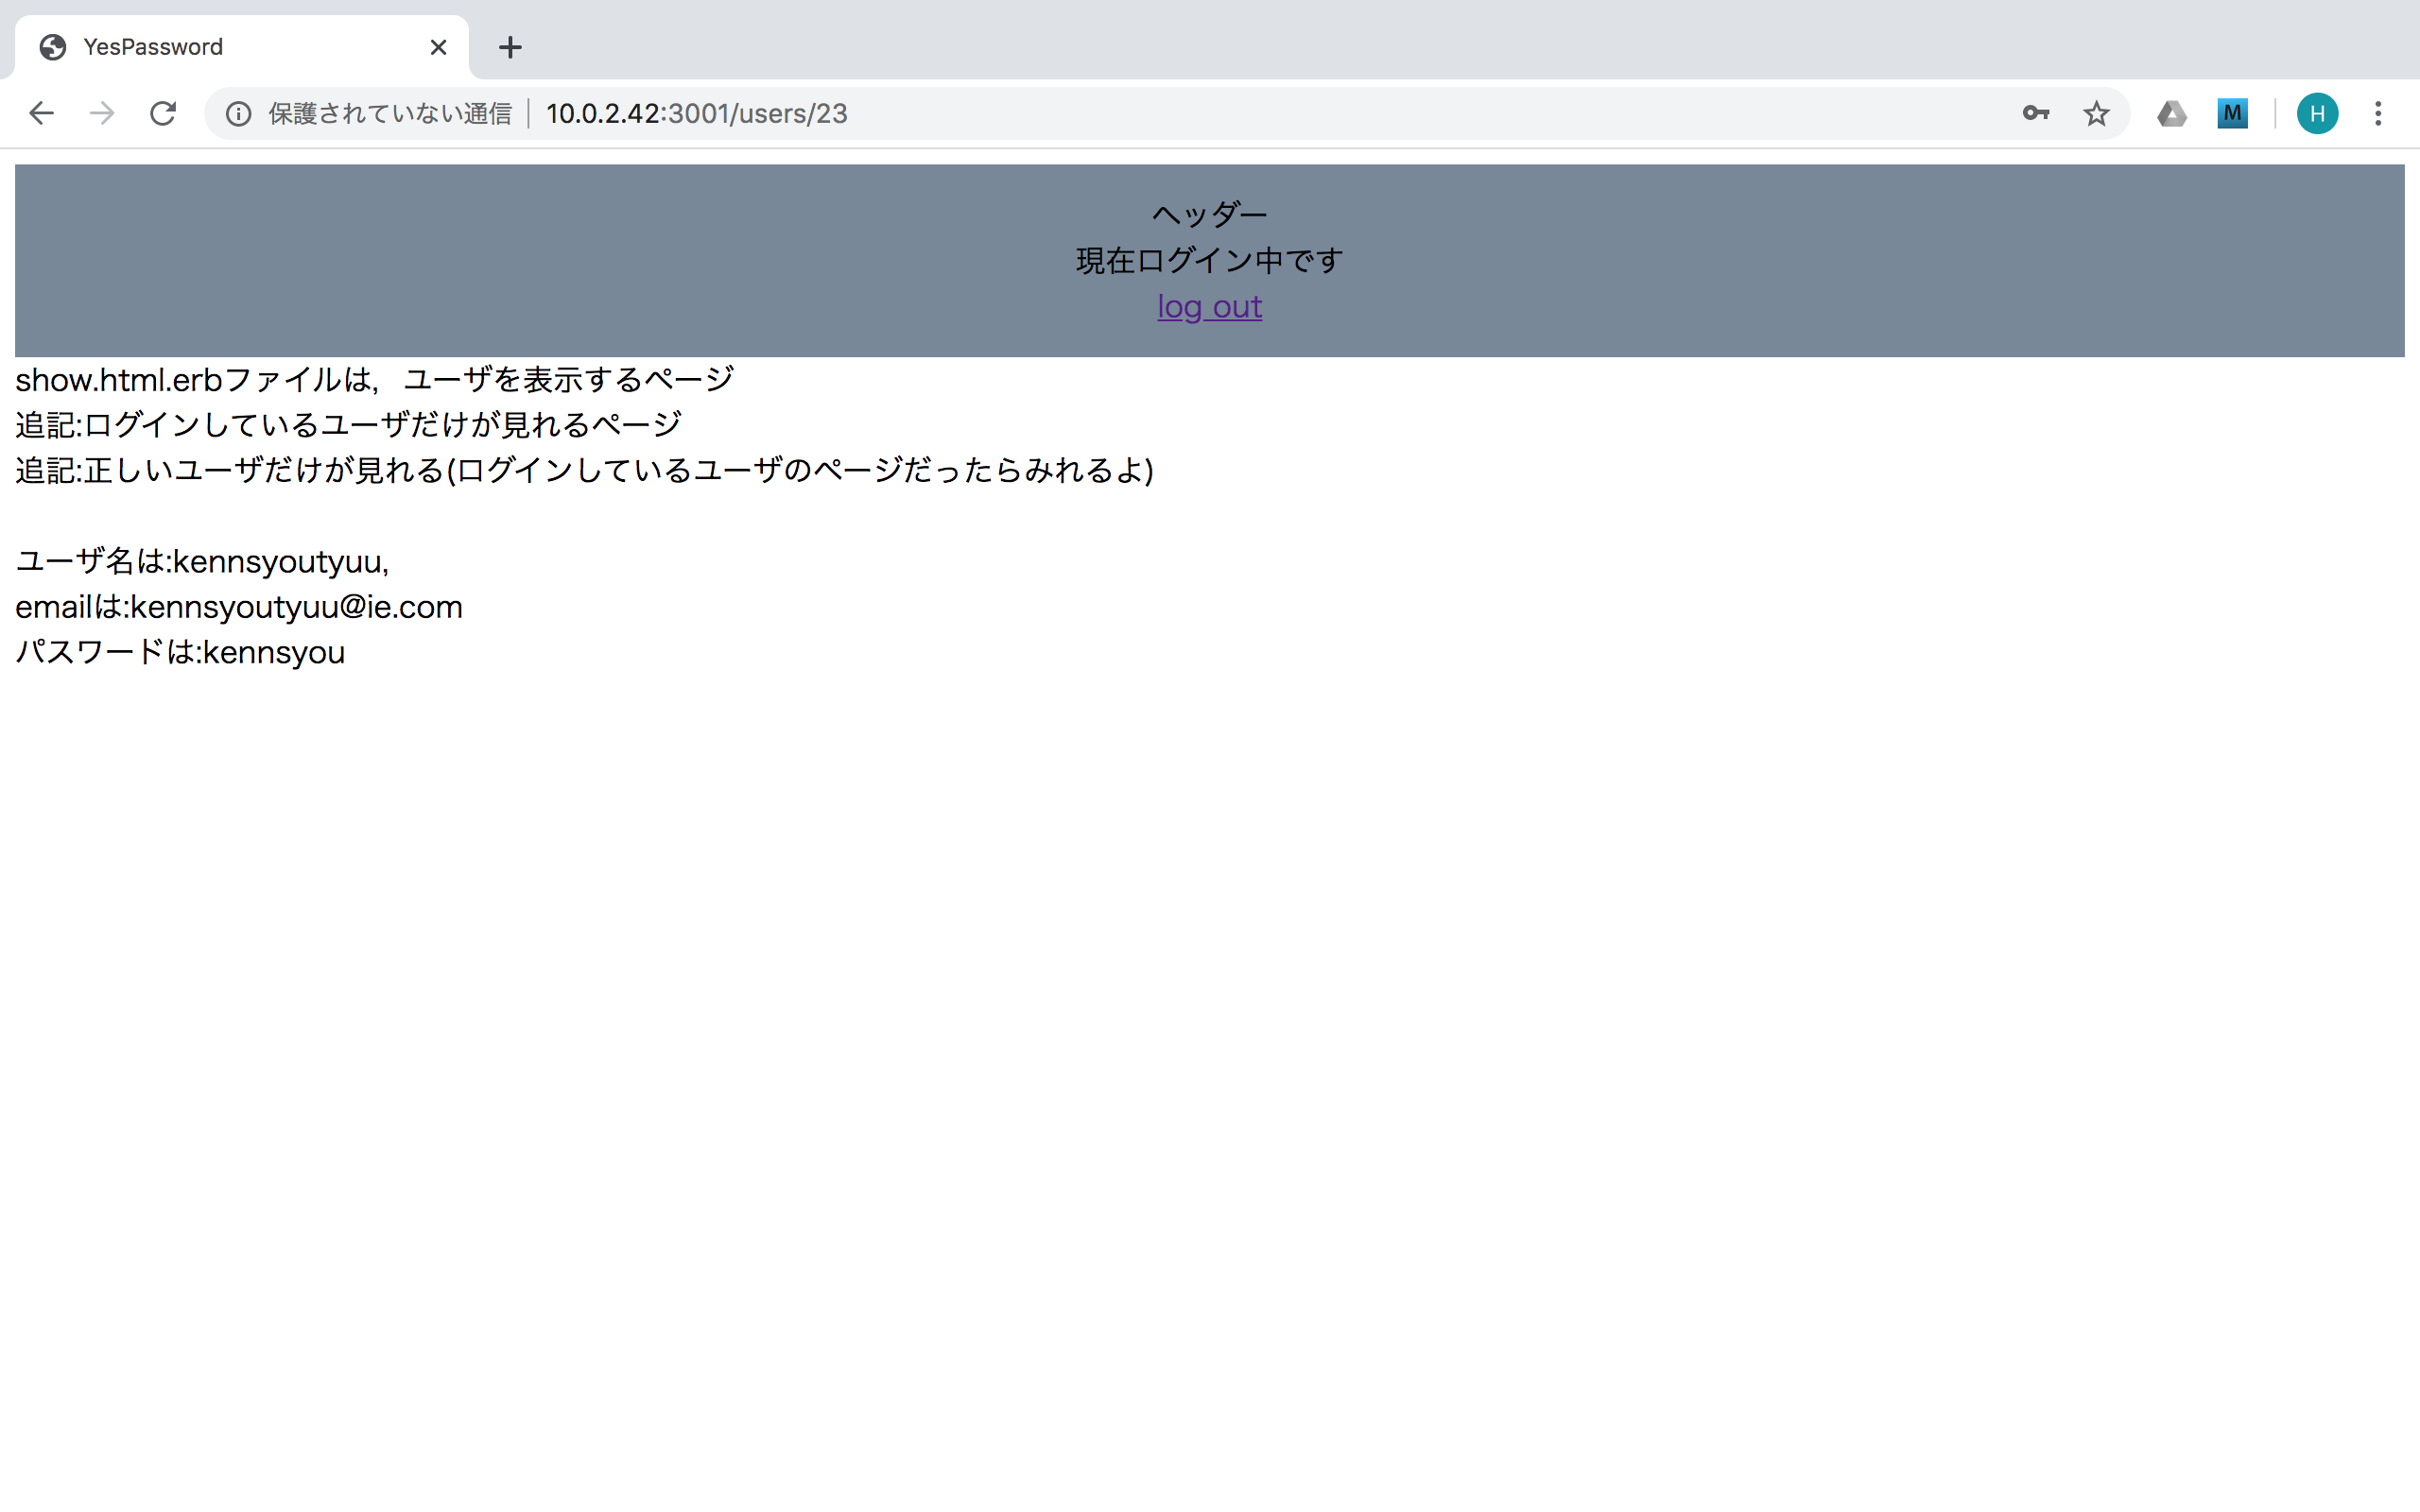
\includegraphics[width=15cm]{./fig/chapter4/inspect_1/password_screnn/success.png}
        \caption{検証1\_認証成功後(パスワード方式)}
        \label{検証1認証成功後(パスワード方式)}
    \end{figure}
    % パスワード方式のスクショ---------------------------








    \newpage
    \newpage

    以下の
    図\ref{検証1アカウント作成(鍵方式)},
    図\ref{検証1認証(鍵方式)}
    図\ref{検証1認証成功後(鍵方式)}
    は,第3章の提案手法で実現した,鍵方式の登録・認証を,実際に被験者に行ってもらった時のブラウザ画面である。
    図\ref{検証1アカウント作成(鍵方式)}は,アカウント登録画面である。
    図\ref{検証1認証(鍵方式)}は,図\ref{検証1アカウント作成(鍵方式)}で登録したアカウントに認証するための画面である。
    図\ref{検証1認証成功後(鍵方式)}は,図\ref{検証1認証(鍵方式)}で認証成功した後の画面である。
    % 鍵方式のスクショ----------------------------------
    \vspace{4cm}%図の位置を正しくする!
    \begin{figure}[H]
        %\centering
        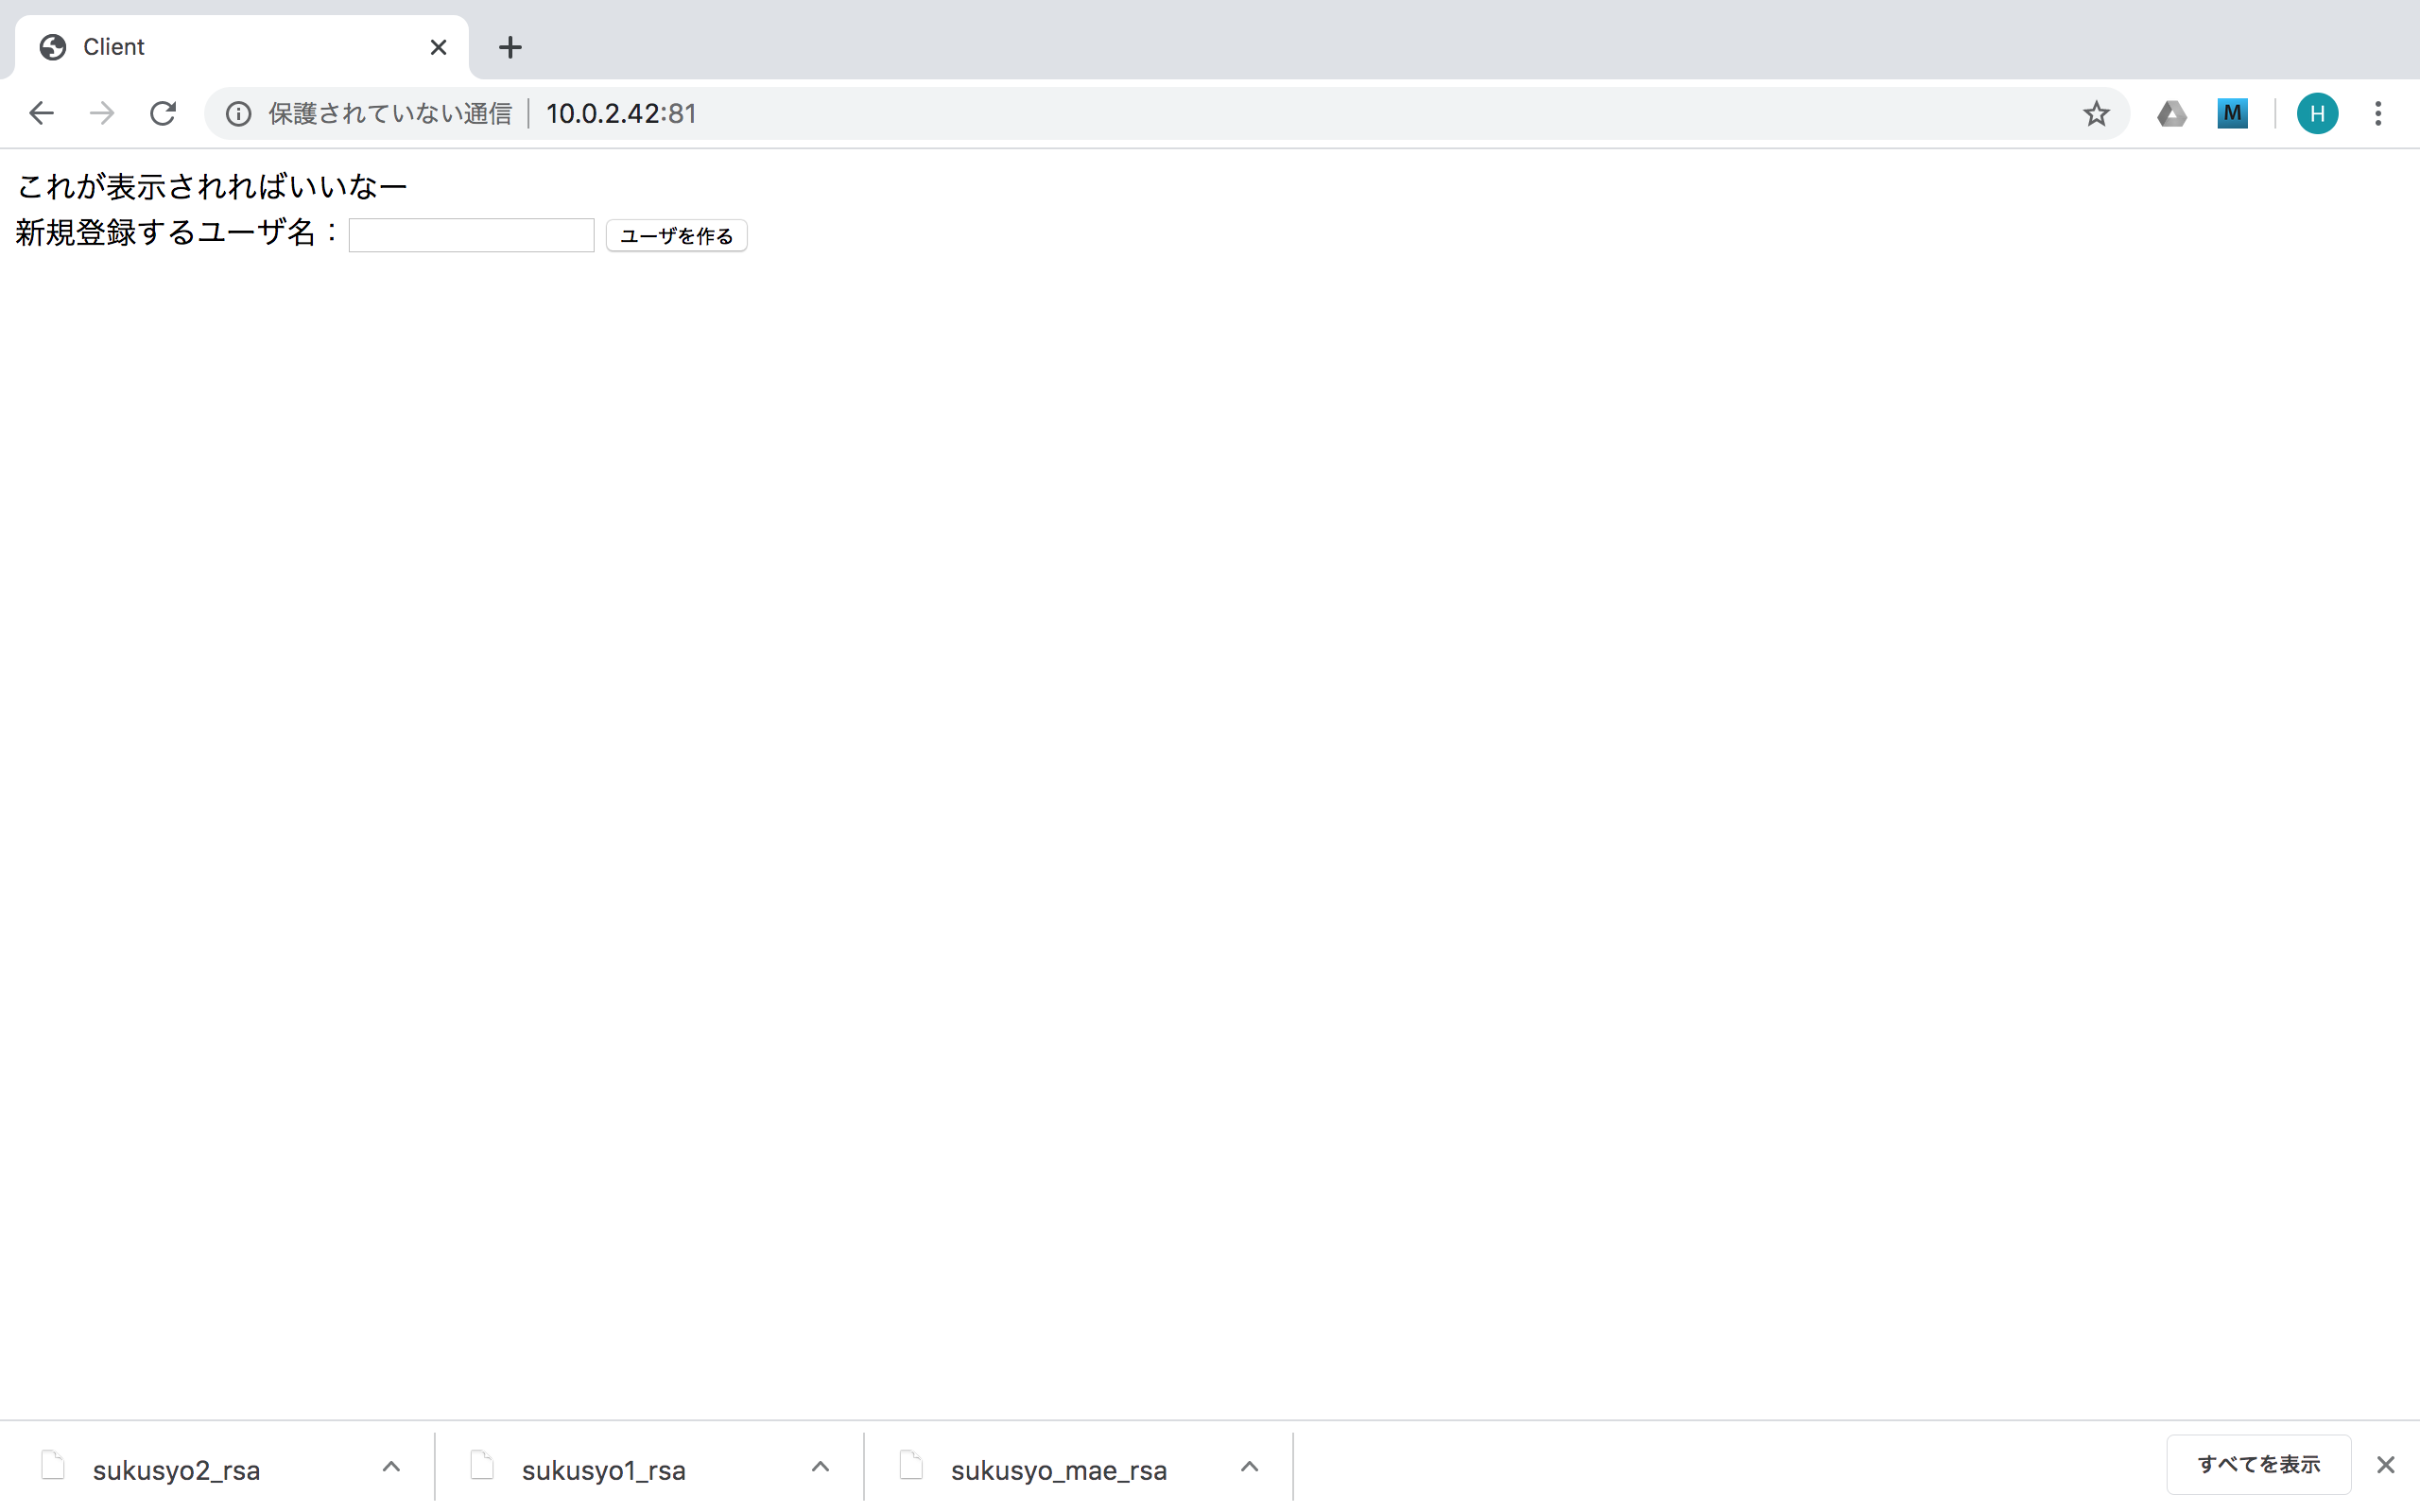
\includegraphics[width=15cm]{./fig/chapter4/inspect_1/key_screnn/sign_up.png}
        \caption{検証1\_アカウント作成(鍵方式)}
        \label{検証1アカウント作成(鍵方式)}
    \end{figure}

    \vspace{4cm}%図の位置を正しくする!
    \begin{figure}[H]
        %\centering
        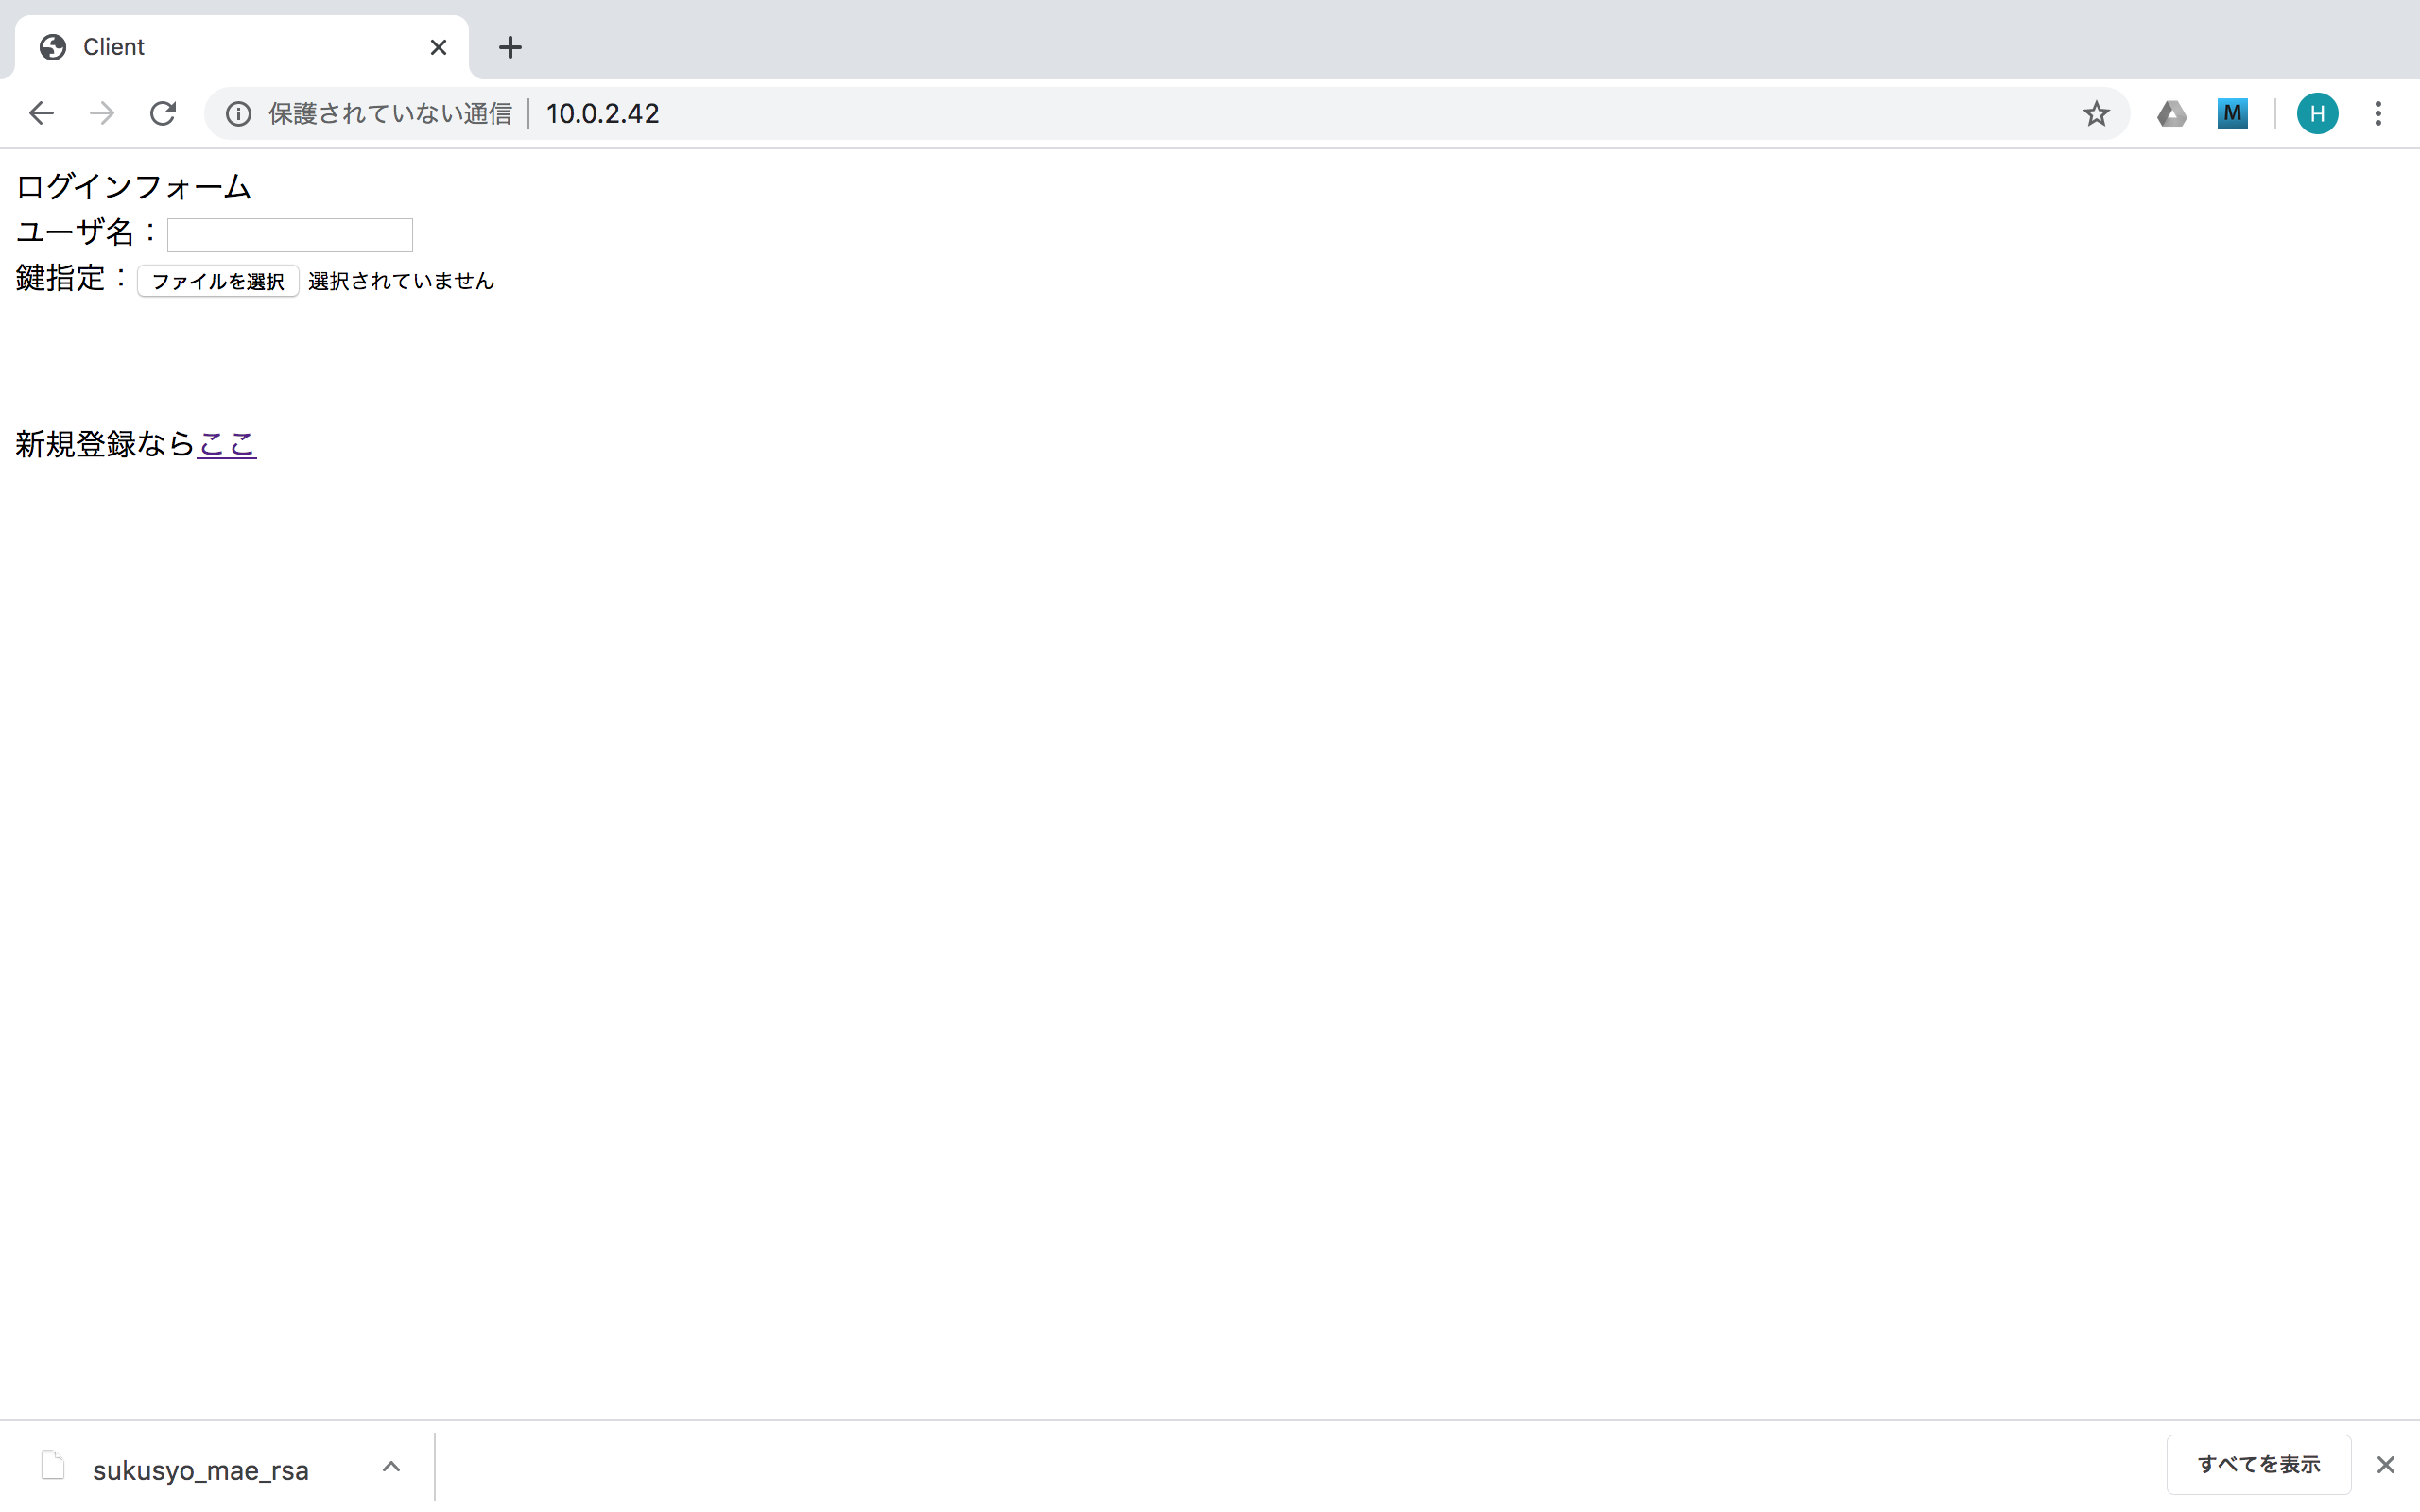
\includegraphics[width=15cm]{./fig/chapter4/inspect_1/key_screnn/login.png}
        \caption{検証1\_認証(鍵方式)}
        \label{検証1認証(鍵方式)}
    \end{figure}

    \vspace{4cm}%図の位置を正しくする!
    \begin{figure}[H]
        %\centering
        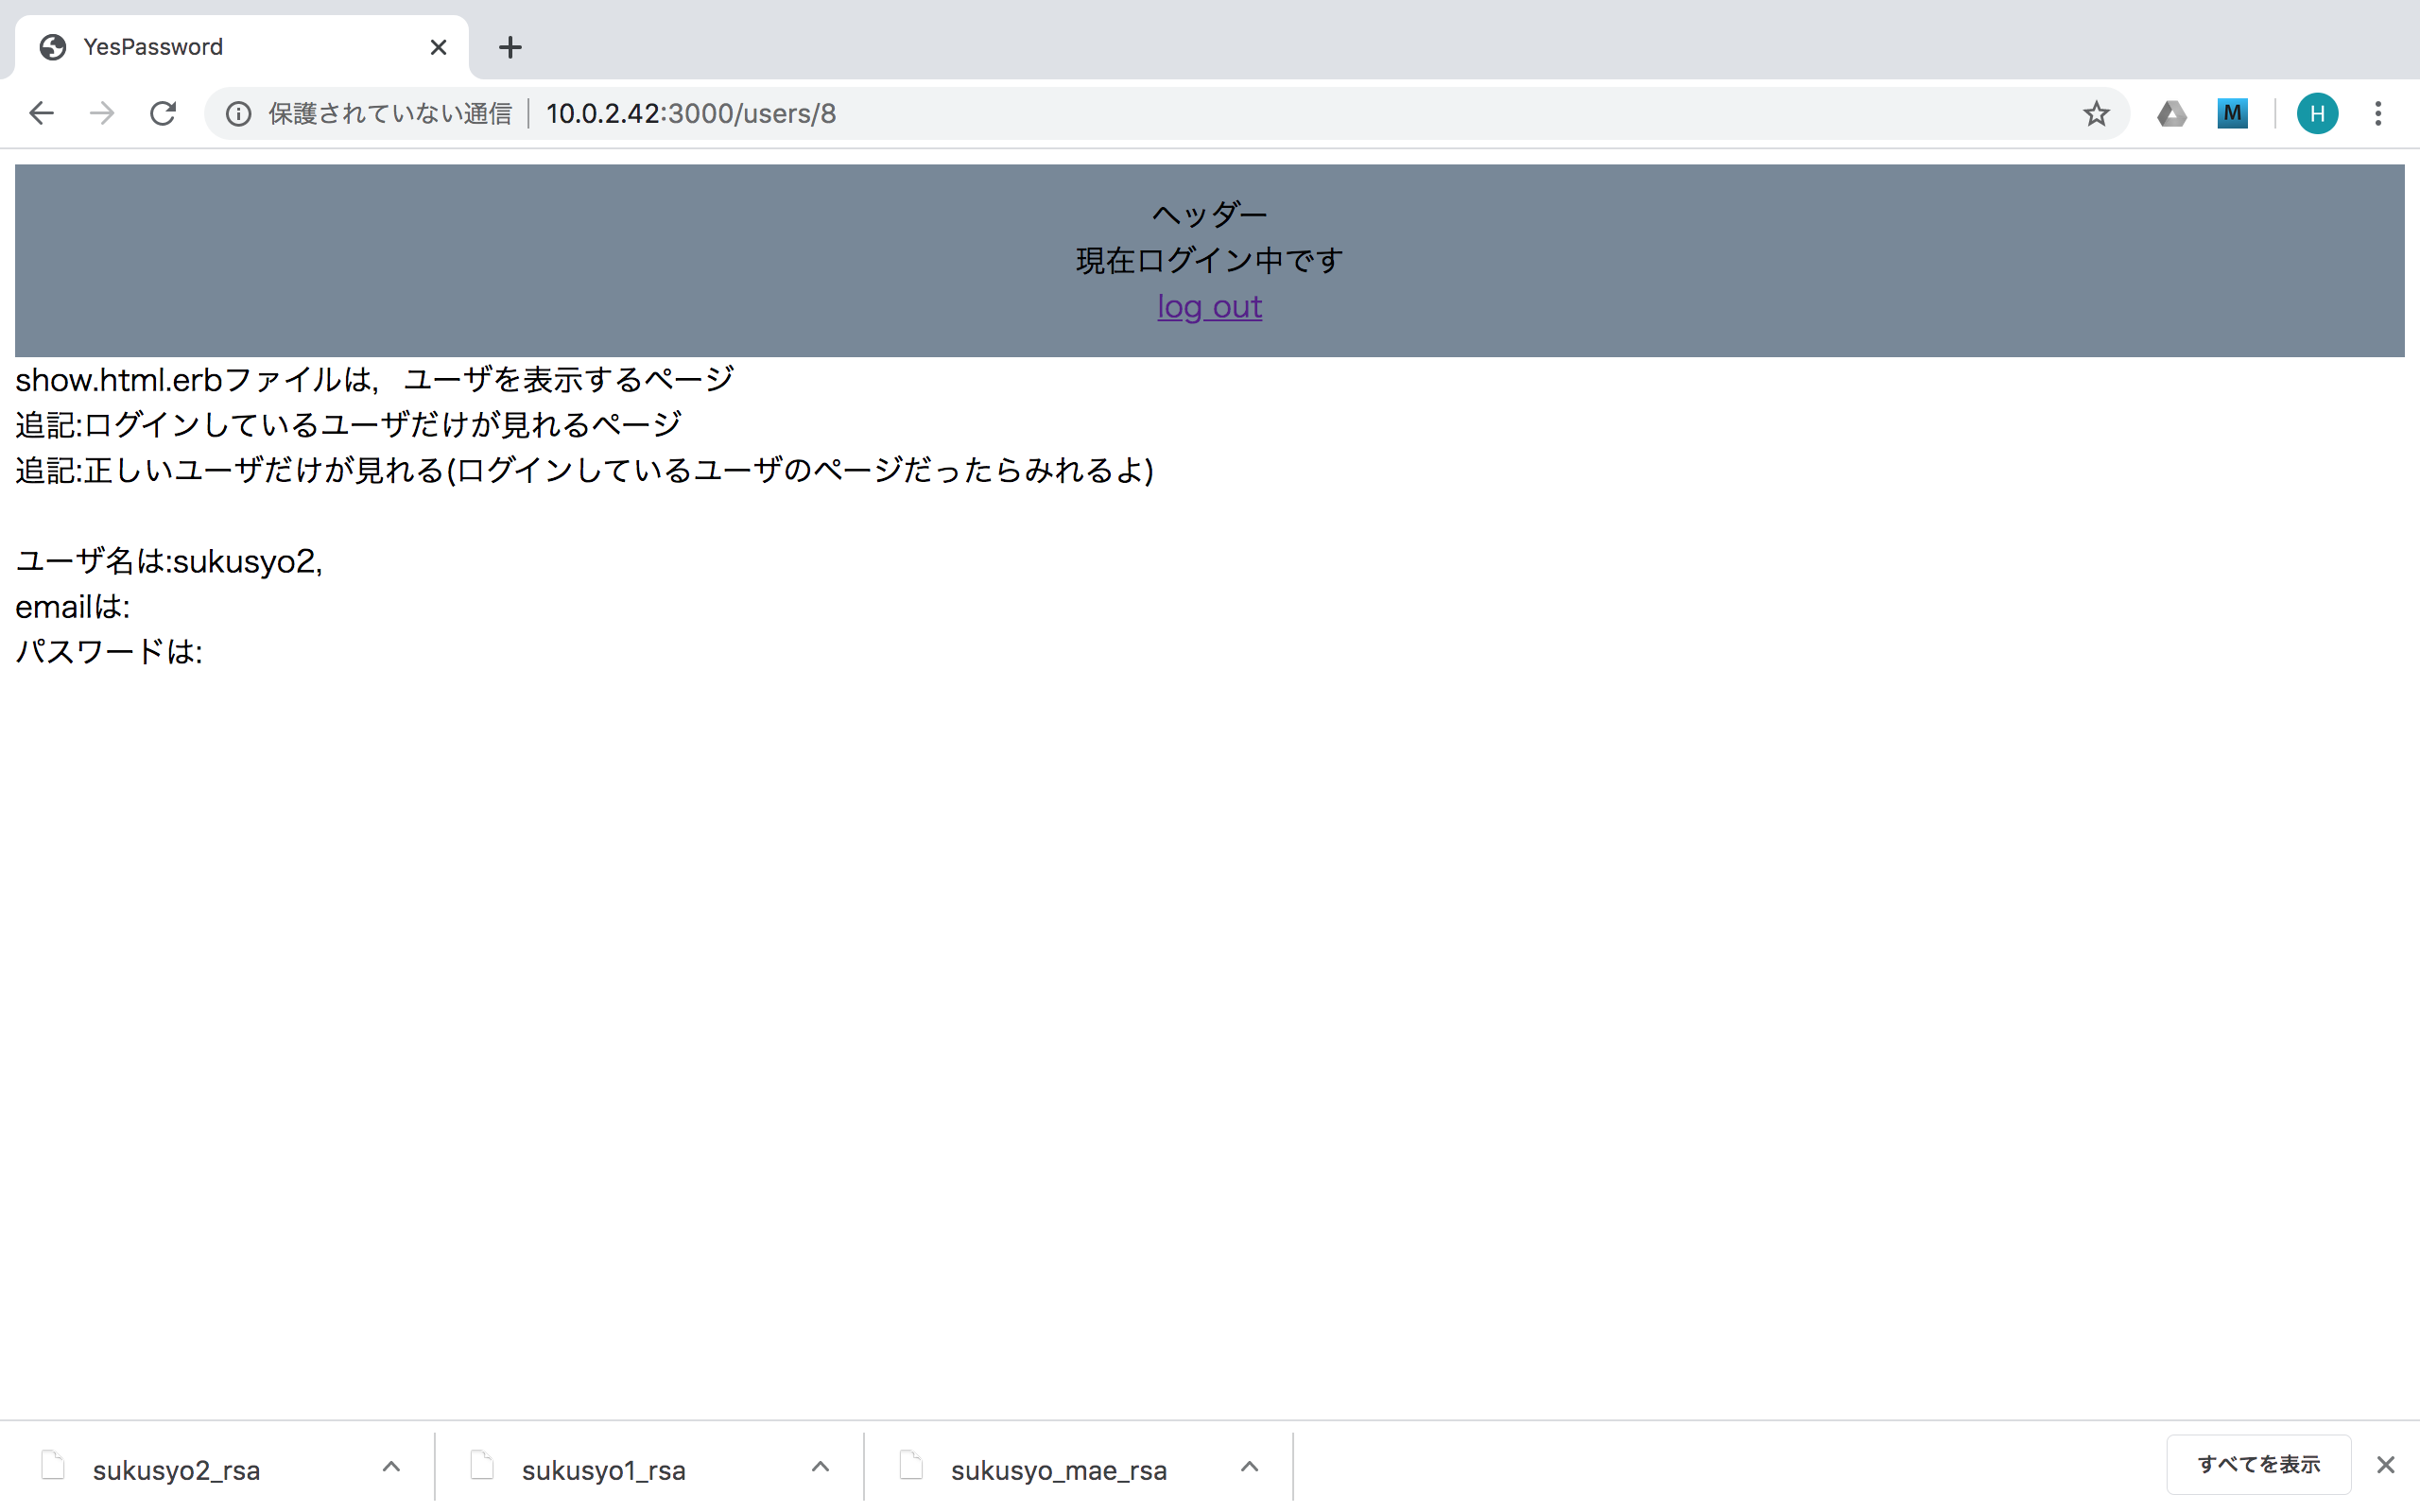
\includegraphics[width=15cm]{./fig/chapter4/inspect_1/key_screnn/login-after2.png}
        \caption{検証1\_認証成功後(鍵方式)}
        \label{検証1認証成功後(鍵方式)}
    \end{figure}
    % 鍵方式のスクショ----------------------------------





    

    以下の
    図\ref{アンケート1},
    図\ref{アンケート2},
    図\ref{アンケート3},
    図\ref{アンケート4}
    は
    図\ref{検証1アカウント作成(パスワード方式)} 〜 図\ref{検証1認証成功後(鍵方式)} までの,
    時間計測が終わった直後に行う,アンケートの画面である。
    %% アンケートの意図を説明
    % 検証自体面倒か
    図\ref{アンケート1} では,"検証自体の面倒さ"をアンケートで聞いている。
    その意図として,"面倒"と感じた感情は,検証役になること自体が面倒だったことに起因していないかを確かめるためである。
    % 登録・認証に対して,面倒と感じた度合いを
    図\ref{アンケート2}では,パスワード方式の登録・認証それぞれについて,どのくらい面倒かを質問している。
    図\ref{アンケート3}では,鍵方式の登録・認証それぞれについて,どのくらい面倒かを質問している。
    図\ref{アンケート2},図\ref{アンケート3}の質問の意図としては,アンケートの観点から"面倒さ"を数値化することである。
    図\ref{アンケート4}では,鍵方式の登録・認証について,被験者の技術視点と利用視点から,自由形式で意見を求めている。
    図\ref{アンケート4}の意図としては,よりよい物を作るために,被験者意見を収集し,今後の方針を決めるためである。

    % アンケートのスクショ----------------------------------
    \vspace{4cm}%図の位置を正しくする!
    \begin{figure}[H]
        %\centering
        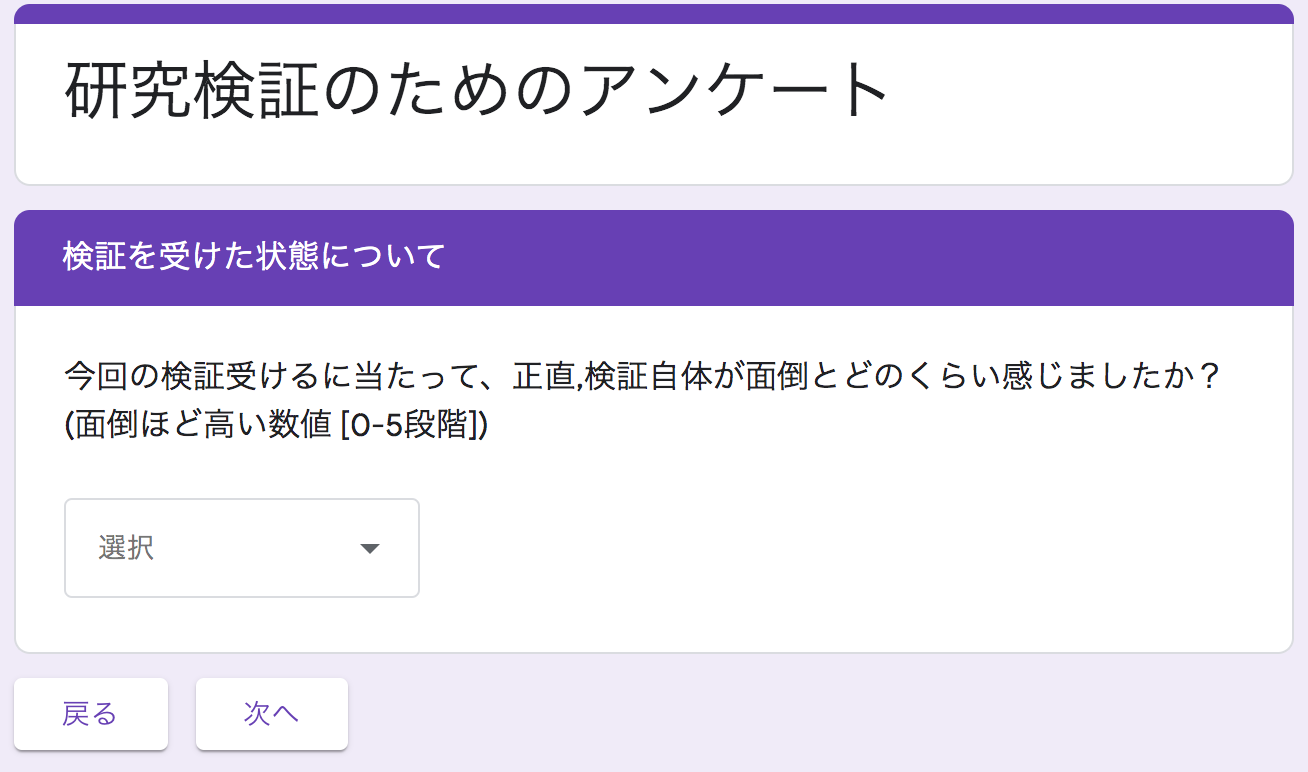
\includegraphics[width=15cm]{./fig/chapter4/inspect_1/questionnaire/questionnaire_1.png}
        \caption{アンケート1}
        \label{アンケート1}
    \end{figure}

    \vspace{4cm}%図の位置を正しくする!
    \begin{figure}[H]
        %\centering
        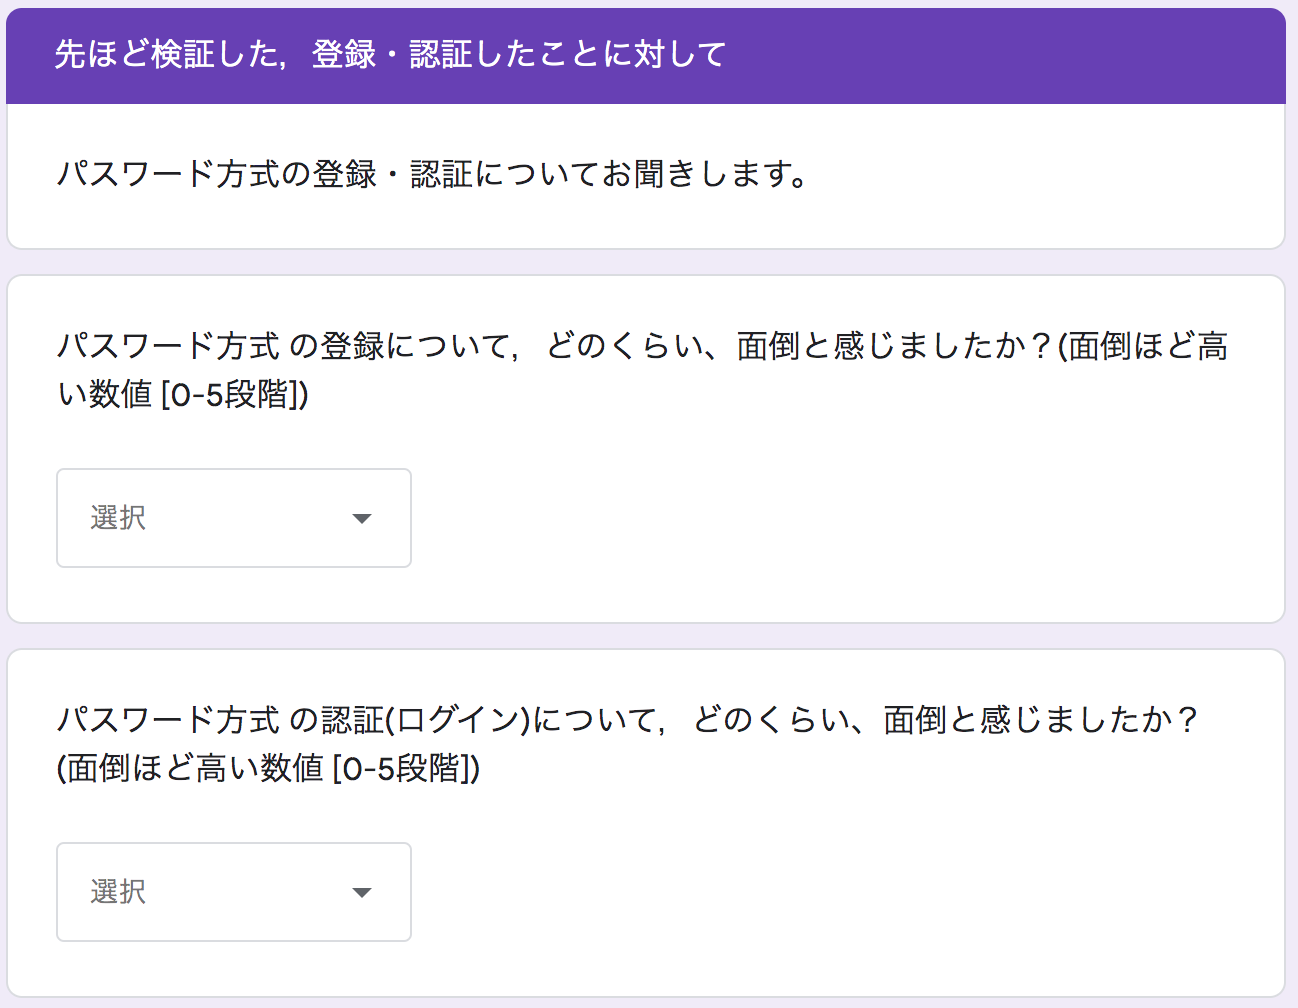
\includegraphics[width=15cm]{./fig/chapter4/inspect_1/questionnaire/questionnaire_2.png}
        \caption{アンケート2}
        \label{アンケート2}
    \end{figure}

    \vspace{4cm}%図の位置を正しくする!
    \begin{figure}[H]
        %\centering
        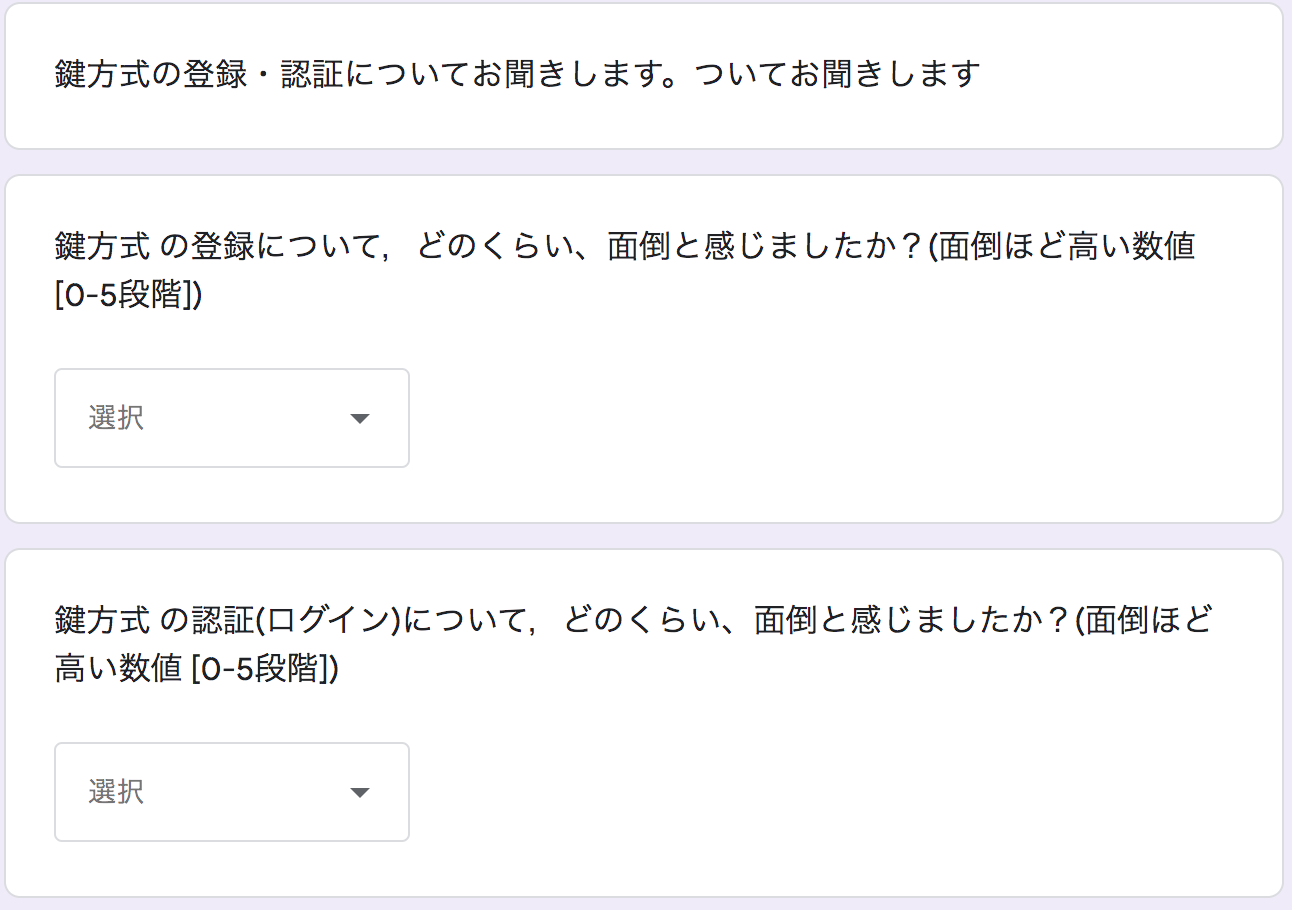
\includegraphics[width=15cm]{./fig/chapter4/inspect_1/questionnaire/questionnaire_3.png}
        \caption{アンケート3}
        \label{アンケート3}
    \end{figure}

    \vspace{4cm}%図の位置を正しくする!
    \begin{figure}[H]
        %\centering
        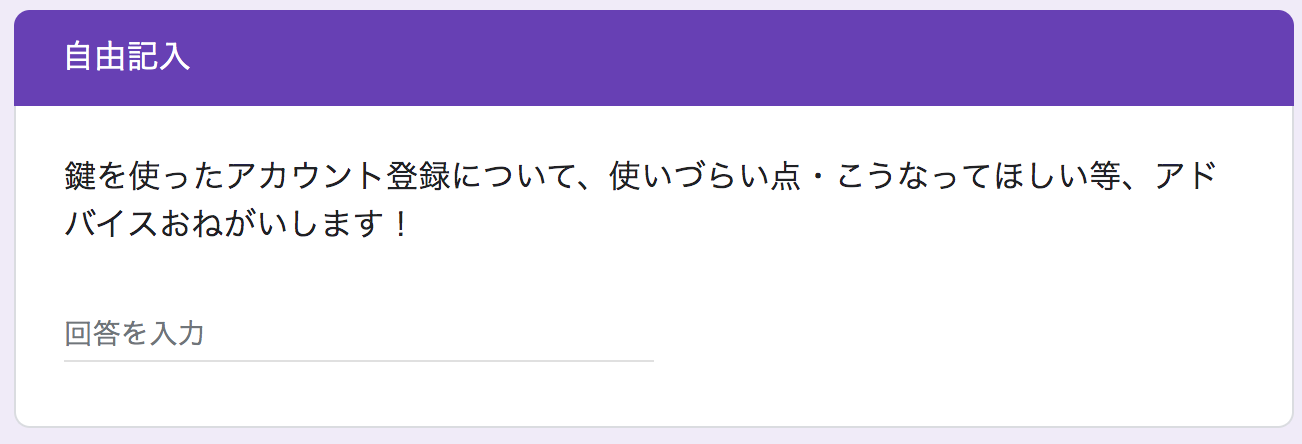
\includegraphics[width=15cm]{./fig/chapter4/inspect_1/questionnaire/questionnaire_4.png}
        \caption{アンケート4}
        \label{アンケート4}
    \end{figure}

    
    % アンケートのスクショ----------------------------------

    %実際に記述--------------------------------------------------------
    




    %%%%%%%%%%%%%%%%%%%%%%%%%%%アン
    %目的
    %  ここでは,被験者に行ったもらう検証画面をのせる。
    %  %(なぜか --> 
    %  % - 検証結果が,どういう検証をした上での,結果になったかを見る必要がある。
    %  % - プラスアルファ
    %  %   - 検証結果を受けて,変更したから,どういう変更したかを,被験者目線でわかるようにする
    %  %)
    %  
    %検証の詳細
    %  パスワード方式の認証・登録の検証画面
    %  鍵方式の認証・登録の検証画面
    %  アンケートの画面
    %
    %  
    %被験者に検証してもらう,鍵方式とパスワード方式それぞれの,登録・認証をする上での,図を載せる。
    %
    %%%%%%%%%%%%%%%%%%%%%%%%%%%アン

 \subsubsection{検証マニュアル}
 %再現性のためにという説明をする
 以下の図\ref{検証マニュアル1},図\ref{検証マニュアル2}は,上記の図\ref{検証1アカウント作成(パスワード方式)} 〜 図\ref{アンケート4} 
 の検証を行うためのマニュアルである.
 マニュアルを作成して,検証を行った意図としては,再現性を持って検証を行うためである.

 \newpage

 \vspace{4cm}%図の位置を正しくする!
 \begin{figure}[H]
     %\centering
     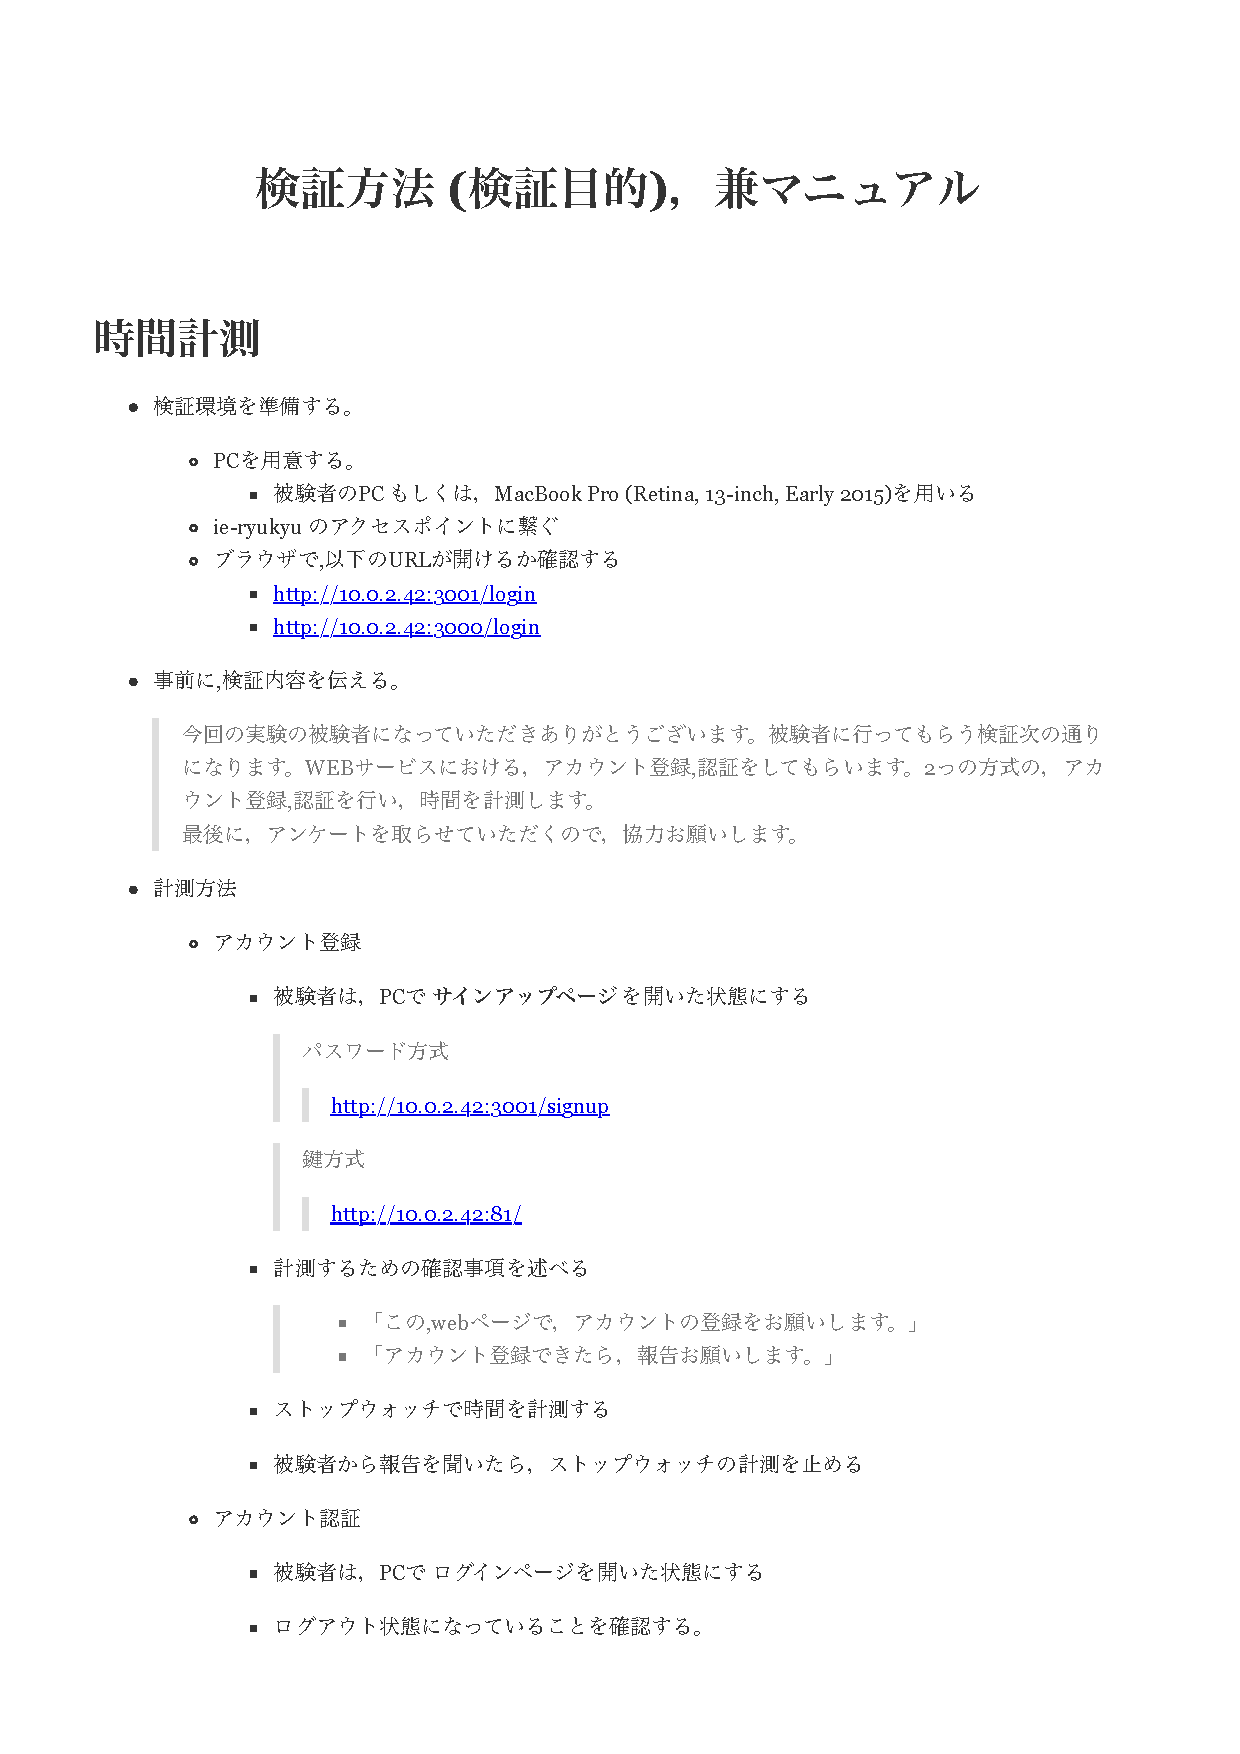
\includegraphics[width=15cm]{./fig/chapter4/inspect_1/manual/manual_1.pdf}
     \caption{検証マニュアル1}
     \label{検証マニュアル1}
 \end{figure}

 \vspace{4cm}%図の位置を正しくする!
 \begin{figure}[H]
     %\centering
     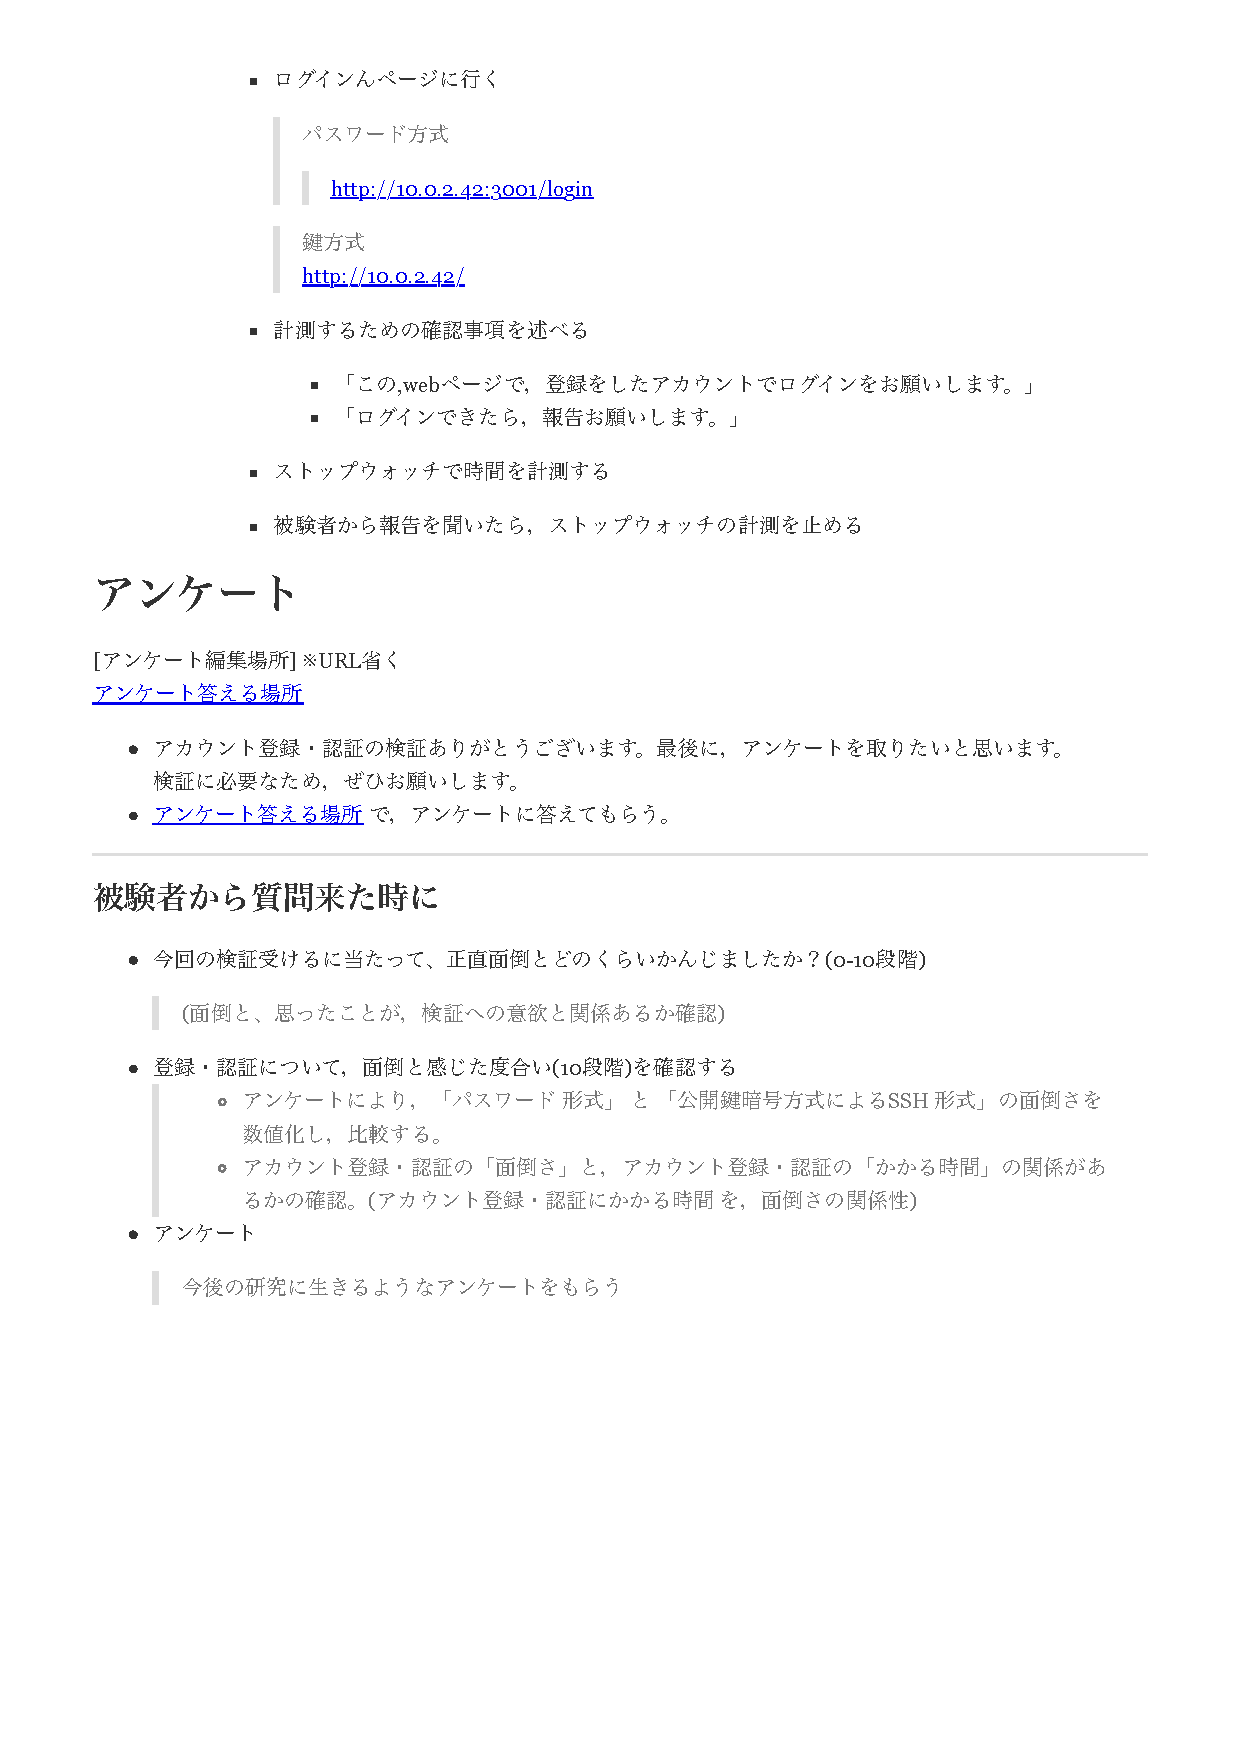
\includegraphics[width=15cm]{./fig/chapter4/inspect_1/manual/manual_2.pdf}
     \caption{検証マニュアル2}
     \label{検証マニュアル2}
 \end{figure}

\subsection{検証結果}
\subsection{考察}

\newpage


\section{検証2}